%
% File acl2014.tex
%
% Contact: koller@ling.uni-potsdam.de, yusuke@nii.ac.jp
%%
%% Based on the style files for ACL-2013, which were, in turn,
%% Based on the style files for ACL-2012, which were, in turn,
%% based on the style files for ACL-2011, which were, in turn, 
%% based on the style files for ACL-2010, which were, in turn, 
%% based on the style files for ACL-IJCNLP-2009, which were, in turn,
%% based on the style files for EACL-2009 and IJCNLP-2008...

%% Based on the style files for EACL 2006 by 
%%e.agirre@ehu.es or Sergi.Balari@uab.es
%% and that of ACL 08 by Joakim Nivre and Noah Smith

\documentclass[11pt]{article}
\usepackage{acl2014}
\usepackage{times}
\usepackage{url}
\usepackage{latexsym}
\usepackage{tikz}
\usepackage{amsmath}
\usepackage{gnuplot-lua-tikz}
\usetikzlibrary{chains,shapes,arrows}
\tikzstyle{textbase} = [text height=1.5ex,text depth=.25ex]


%\setlength\titlebox{5cm}

% You can expand the titlebox if you need extra space
% to show all the authors. Please do not make the titlebox
% smaller than 5cm (the original size); we will check this
% in the camera-ready version and ask you to change it back.


\title{Faster Phrase-Based Decoding by Refining Feature State}

\author{}

\date{}

\begin{document}
\maketitle
\begin{abstract}
We contribute a faster decoding algorithm for phrase-based machine translation.  Translation hypotheses keep track of state, such as context for the language model and coverage of words in the source sentence.  Most features depend upon only part of the state, but traditional algorithms, including cube pruning, handle state atomically.  For example, cube pruning will repeatedly query the language model with hypotheses that differ only in source coverage, despite the fact that source coverage is irrelevant to the language model.  
Our algorithm avoids this behavior by placing hypotheses into equivalence classes, masking the parts of state that matter least to the score.  
Since our algorithm and cube pruning are both approximate, the improvement can be used to increase speed or accuracy.  
%TODO result
When tuned to attain the same accuracy, our algorithm is OVER 9000 times as fast as the Moses decoder with cube pruning.  
\end{abstract}

\section{Introduction}
\label{intro_label}
Translation speed is critical to making suggestions as translators type, mining for parallel data by translating the web, and running on mobile devices without Internet connectivity.  We contribute a fast decoding algorithm for phrase-based machine translation along with an implementation in a new open-source (LGPL) decoder.  

Phrase-based decoders \cite{moses,phrasal,jane-phrase} keep track of several types of information with translation hypotheses: coverage of the source sentence thus far, context for the language model, and state for other features.  Existing decoders treat this information as atomic: hypotheses that have exactly the same information can be recombined and efficiently handled via dynamic programming, but there is no special handling for two hypotheses that have the same language model context.  Therefore, the language model is repeatedly consulted regarding hypotheses that differ only in ways irrelevant to its score, such as coverage of the source sentence.  Our decoder bundles hypotheses into equivalence classes that allow the language model to focus solely on the words that matter to its score.  

Like most phrase-based decoders \cite{pharaoh}, hypotheses are built from left to right by appending phrases in the target language.  When this happens, the language model uses the last $N-1$ words of the hypothesis as context to score the first $N-1$ words of the phrase, where $N$ is the order of the model.  Traditional decoders \cite{cubit} try thousands of combinations of hypotheses and phrases, hoping to find ones that the language model likes.  Our algorithm instead discovers good combinations in a coarse-to-fine manner inspired by \newcite{search}, which presented a decoding algorithm for syntactic machine translation.  The algorithm exploits the fact that hypotheses often share the same suffix and phrases often share the same prefix.  These shared suffixes and prefixes allow the algorithm to coarsely reason over many combinations at once.   

%The algorithm starts by examining boundary words: the last word of each hypothesis and the first word of each phrase.  Options that score well together are refined by examining additional words from hypotheses with matching suffixes and phrases with matching prefixes.  This refinement process continues until some combinations have been fully scored by examining all $2N-2$ relevant words.    

As with most search algorithms for phrase-based machine translation, our algorithm is approximate.  One can trade between CPU time and search accuracy by choosing how many hypotheses to keep in each step of the search.  The primary claim is that our algorithm offers a better trade-off between time and accuracy when compared with the popular cube pruning algorithm \cite{cubit}.  

\section{Related Work}
Part of our phrase-based decoding algorithm is inspired by the syntactic decoding algorithm of \newcite{search}.  Their work exploited common prefixes and suffixes of translation hypotheses in order to efficiently reason over many hypotheses at once.  In some sense, phrase-based translation is simpler because hypotheses are constructed from left to right, so there is no need to worry about the prefix of a hypothesis.  However, this simplification comes with a different cost: phrase-based translation implements reordering by allowing hypotheses to correspond to discontiguous words in the source sentence.  There are exponentially many ways to cover the source sentence, so we developed an efficient way for the language model to reason over hypotheses that cover different parts of the source sentence.  In contrast, syntactic machine translation hypotheses correspond to contiguous spans in the source sentence, so \newcite{search} simply ran their algorithm separately in every possible span.  

Another difference from \newcite{search} is that they made no effort to exploit common words that appear in translation rules, which in our case are analogous to phrases.  In this work, we explicitly group target phrases by common prefixes, doing so directly in the phrase table.  

Coarse-to-fine approaches \cite{coarsetofine,coarsetofineorig} invoke the decoder multiple times with increasingly detailed models, pruning after each pass.  The key difference in our work is that, rather than refining models in lock step, we effectively refine the language model on demand for hypotheses that score well.  Moreover, their work was performed in syntactic machine translation while we address issues specific to phrase-based translation.  

Our baseline is cube pruning, which was originally developed for syntactic machine translation \cite{cubepruning} and subsequently ported to phrase-based translation by \newcite{cubit}.  We have largely adopted their search strategy, which we summarize in Section \ref{basic_search}.  However, as noted in Section \ref{intro_label}, cube pruning repeatedly calls the language model regarding hypotheses that differ only in coverage, while we collapse these calls.  Moreover, we take a coarse-to-fine approach to finding good combinations of hypotheses and phrases rather than simply trying a large number of them.  

\newcite{lagrangian-phrase} developed an exact decoding algorithm based on Lagrangian relaxation.  However, they experimented with trigram language models and it remains unclear whether their algorithm would tractably handle the 5-gram language models used by many modern machine translation systems.  We evaluate our approximate search algorithm using a 5-gram language model.  

\section{Decoding}
We begin by summarizing the high-level organization of phrase-based cube pruning in Moses \cite{moses}, which is largely based upon Cubit \cite{cubit}, and in turn based upon Pharaoh \cite{pharaoh}.  Sections \ref{contribution} and later show our contribution.  

\subsection{Search Organization}
\label{basic_search}
Phrase-based decoders construct hypotheses from left to right by appending phrases in the target language.  The decoder organizes this search process using \emph{stacks}.  Shown in Figure~\ref{stacks}, stacks contain hypotheses that have translated the same number of source words.  The zeroth stack contains a single hypothesis that has translated nothing.  The decoder extends this hypothesis by translating one source word, producing a stack containing several competing hypotheses.  Hypotheses remember which source word they translated, as indicated by the filled circles.  The decoder then proceeds to search for hypotheses that translate two words of the source sentence.  This can be accomplished by extending the zeroth stack with a two-word source phrase or by extending the preceding stack with a one-word source phrase.  Returning to the example in Figure~\ref{stacks}, the decoder can apply a phrase pair to translate ``le chat'' as ``cat'' or it can derive ``the cat'' by translating one word at a time.  To generalize, the decoder populates the $i$th stack by pairing hypotheses in the $i-j$th stack with target phrases that translate source phrases of length $j$.  

%the decoder produces a stack of hypotheses that have translated two words.  It can do so by translating another source word or by translating two source words at once using a longer phrase.  For example, Figure~\ref{stacks} shows a hypothesis that used a phrase to translate ``le chat'' as ``cat'', thereby covering two source words at once.  
  
\newcommand{\csiz}{1.5pt}
\newcommand{\copen}{\node[draw,on chain,circle,inner sep=\csiz] {};}
\newcommand{\cfull}{\node[draw,on chain,circle,fill=black,inner sep=\csiz] {};}
\newcommand{\cov}[2]{\begin{tikzpicture}[start chain,node distance=1pt]#1\node[on chain,textbase]{#2};\end{tikzpicture}}
\newcommand{\clin}{\\[-5pt]}

\begin{figure}\small%
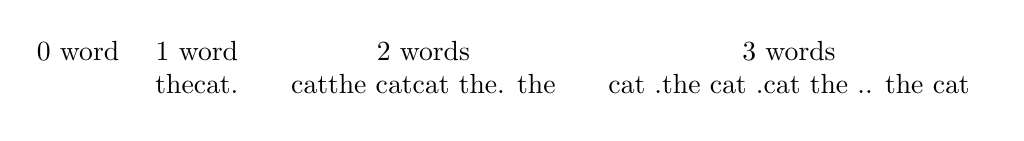
\begin{tikzpicture}
\node (h0) {\begin{tabular}{@{}c@{}}
0 word\\
\cov{\copen\copen\copen}{}
\end{tabular}};
\node[right=0pt of h0.north east,anchor=north west] (h1) {\begin{tabular}{l}
\multicolumn{1}{c}{1 word}\\
\cov{\cfull\copen\copen}{the}\clin
\cov{\copen\cfull\copen}{cat}\clin
\cov{\copen\copen\cfull}{.}\clin
\end{tabular}};
\node[right=0pt of h1.north east,anchor=north west] (h2){\begin{tabular}{l}
\multicolumn{1}{c}{2 words}\\
\cov{\cfull\cfull\copen}{cat}\clin
\cov{\cfull\cfull\copen}{the cat}\clin
\cov{\cfull\cfull\copen}{cat the}\clin
\cov{\cfull\copen\cfull}{. the}\clin
\end{tabular}};
\node[right=0pt of h2.north east,anchor=north west] (h3){\begin{tabular}{l}
\multicolumn{1}{c}{3 words}\\
\cov{\cfull\cfull\cfull}{cat .}\clin
\cov{\cfull\cfull\cfull}{the cat .}\clin
\cov{\cfull\cfull\cfull}{cat the .}\clin
\cov{\cfull\cfull\cfull}{. the cat}\clin
\end{tabular}};
\end{tikzpicture}
\caption{\label{stacks}Stacks to translate the French ``le chat .'' into English.  Filled circles indicate that the source word has been translated.  A phrase translates ``le chat'' as simply ``cat'', emphasizing that stacks are organized by the number of source words rather than the number of target words.}
\end{figure}

In practice, the decoder enforces a reordering limit that prevents the search process from jumping around the source sentence too much and dramatically reduces the size of the search space.  Formally, when the reordering limit is $R$, the decoder must translate source words at indices $[0,n-R)$ before, or at the same time as, it can translate the $n$th source word.  

The second practical constraint is a limit on the number of hypotheses in each stack.  There are generally too many possible hypotheses, so the decoder approximates by remembering at most $k$ hypotheses in each stack, where $k$ is a number chosen by the user.  Small $k$ makes search fast but may prune good hypotheses, while large $k$ is more thorough but takes more CPU time, thereby comprising a time-accuracy trade-off.  The central question in this paper is how to select these $k$ hypotheses while improving the time-accuracy trade-off.  

%To formalize the preceding paragraph, stack $s_i$ is a set of hypotheses that have translated $i$ source words.  The initial stack $s_0$ contains a single hypothesis that translates nothing while the subsequent stacks are defined inductively
%\[s_i = \bigcup_{j=0}^{i-1} \text{extend}(s_j, \text{source}_{i-j}) \]
Populating a stack can be boiled down into two steps.  In the first step, the decoder matches hypotheses with source phrases subject to three constraints: the total source length matches the stack being populated, none of the source words has already been translated by the hypothesis, and the reordering limit.  We do not improve this first step, which is largely driven by checking whether a hypothesis and source phrase are compatible along with some knowledge about the reordering limit.  In the second step, the decoder runs an algorithm that searches through these matches to select $k$ high-scoring hypotheses for placement in the stack.  We improve this second step.   

%First, the decoder matches hypotheses with source phrases that they have yet to translate and that will meet the source length requirement of the stack.  The purpose of the reordering limit is to substantially reduce the size of the search space to make search tractable and as a workaround for models that are too weak to handle long-distance reordering.  Second, the decoder searches through 

%Second, the decoder searches through these matches for good pairings 
The decoder provides our algorithm with pairs consisting of a hypothesis and a compatible source phrase.  Each source phrase translates to multiple compatible target phrases.  The task is to grow these hypotheses by appending a compatible target phrase, yielding a new hypothesis.  These new hypotheses will be placed into a stack of size $k$, so we are interested in selecting $k$ new hypotheses that score highly.  The user chooses parameter $k$.

Beam search \cite{beam-speech,pharaoh} takes a brute force approach: try every hypothesis with every compatible target phrase then select the top $k$ new hypotheses by score.  This seems wasteful because most hypotheses are discarded.  Instead, we follow cube pruning \cite{cubepruning} in using a priority queue to generate $k$ hypotheses.  The key difference is that we generate these hypotheses iteratively rather than atomically.  

%To formalize the problem, we want to extract $k$ high-scoring hypotheses from the set
%\[\{\text{append}(h, t): (h,s) \in \text{input}, t \in \text{target}(s) \}\]
%where $h$ denotes a hypothesis, $t$ denotes a target phrase, $s$ denotes a source phrase, and the input was provided by the decoder.  We begin by grouping the hypotheses according to the source phrase
%\[\bigcup_s \{\text{append}(h, t): (h,s) \in \text{input}, t \in \text{target}(s) \}\]


\subsection{Tries}
\label{contribution}
For each source phrase, we collect the set of compatible hypotheses.  We then place these hypotheses in a trie that emphasizes the suffix words because these matter most when appending a target phrase.  Figure~\ref{hypsuff} shows an example.  While it suffices to build this trie on the last $N-1$ words that matter to the language model, \newcite{zhifei} have shown that fewer words are necessary in cases where the language model will provably back off.  Therefore, the trie does not necessarily have uniform depth.  The leaves of the trie are complete hypotheses and reveal information irrelevant to the language model, such as coverage of the source sentence and the state of other features.  

\begin{figure}\centering
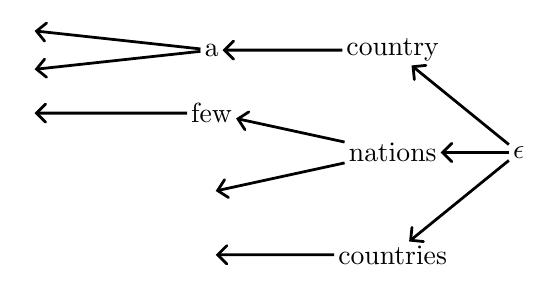
\begin{tikzpicture}[grow=left,->,arrows={-angle 90},line width=1pt,inner sep=1pt]
\tikzstyle{level 1}=[level distance=1.6cm, sibling distance=1.3cm]
\tikzstyle{level 2}=[level distance=2.3cm, sibling distance=1cm]
\tikzstyle{level 3}=[level distance=2.3cm, sibling distance=0.5cm]
\node{$\epsilon$}
child {
  node {country}
  child {
    node{a}
    child {
      node{\cov{\cfull\copen\cfull\copen}{}}
    }
    child {
      node{\cov{\cfull\cfull\copen\copen}{}}
    }
  }
}
child {
  node {nations}
  child {
    node {few}
    child {
      node{\cov{\cfull\copen\cfull\copen}{}}
    }
  }
  child {
%    node {several}
%    child {
      node{\cov{\cfull\copen\cfull\copen}{}}
%    }
  }
}
child {
  node {countries}
  child {
    node{\cov{\cfull\cfull\copen\copen}{}}
  }
}
;
\end{tikzpicture}
\caption{\label{hypsuff}Hypothesis suffixes arranged into a trie.  The leaves indicate source coverage and any other hypothesis state.}
\end{figure}

Each source phrase translates to a set of target phrases.  Because these phrases will be appended to a hypothesis, the first few words matter the most to the language model.  We therefore arrange the source phrases into a prefix trie.  An example is shown in Figure~\ref{tgtpre}.  Similar to the hypothesis trie, the depth may be shorter than $N-1$ in cases where the language model will provably back off \cite{zhifei}.  The trie can also be short because the target phrase has fewer than $N-1$ words.  We currently store this trie data structure directly in the phrase table, though it could also be computed on demand to save memory.  Empirically, our phrase table uses less RAM than Moses's memory-based phrase table.  

\begin{figure}\centering
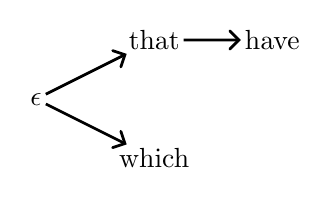
\begin{tikzpicture}[grow=right,->,arrows={-angle 90},line width=1pt,inner sep=1pt]
\node{$\epsilon$}
child {
  node {which}
}
child {
  node {that}
  child {
    node {have}
  }
}
;
\end{tikzpicture}
\caption{\label{tgtpre}Target phrase prefixes arranged into a trie.}
\end{figure}

As an optimization, a trie reveals multiple words when there would otherwise be no branching.  This allows the search algorithm to make decisions only when needed.  

Following \newcite{search}, leaves in the trie take the score of the underlying hypothesis or target phrase.  If there are multiple target phrases with the same language model prefix, we take the highest score.  Nodes higher in the trie take the maximum score of their descendants.   Children of a node are sorted by score.   

\subsection{Boundary Pairs}
The idea is that the decoder reasons over pairs of nodes in the hypothesis and phrase tries before devling into detail.  In this way, it can determine what the language model likes and, conversely, quickly discard combinations of words that the model does not like.  

A boundary pair consists of a node in the hypothesis trie and a node in the target phrase trie.  For example, the decoder starts at the root of each trie with the boundary pair $(\epsilon, \epsilon)$.  The score of a boundary pair is the sum of the scores of the underlying trie nodes.  However, once some words have been revealed, the decoder calls the language model to compute a score adjustment.  For example, the boundary pair $(\text{country}, \text{that})$ has score adjustment
\[\log \frac{p(\text{that}\mid\text{country})}{p(\text{that})} \]
times the weight of the language model.  This has the effect of cancelling out the estimate made when the phrase was scored in isolation and replacing the estimate with a more accurate one based on available context.  These score adjustments are efficient to compute because the decoder retains a pointer to the entry for ``that'' in the language model's data structure \cite{iwslt}. 

\subsection{Splitting}
Refinement is the notion that the boundary pair $(\epsilon, \epsilon)$ divides into several boundary pairs that reveal specific words from hypotheses or target phrases.  The most straightforward way to do this is simply to split into all children of a trie node.  Continuing the example from Figure~\ref{hypsuff}, we could split $(\epsilon, \epsilon)$ into three boundary pairs: $(\text{country}, \epsilon)$, $(\text{nations}, \epsilon)$, and $(\text{countries}, \epsilon)$.  However, it is somewhat inefficient to separately consider the low-scoring child $(\text{countries}, \epsilon)$.  Instead, we continue to split off the best child $(\text{country}, \epsilon)$ and leave a note that the zeroth child has been split off, denoted $(\epsilon[1^+], \epsilon)$.  The index increases each time a child is split off.  

For purposes of scoring, the best child no longer counts as a descendant of $(\epsilon[1^+], \epsilon)$, so its score decreases.    

Splitting alternates sides, so splitting $(\text{countries}, \epsilon)$ will reveal a word from the target phrase.  The exception is that language model scores are completely resolved before hypotheses reveal coverage vectors and other feature state.  

\begin{figure*}[t]%
\hspace{-20pt}\begin{tabular}{l}
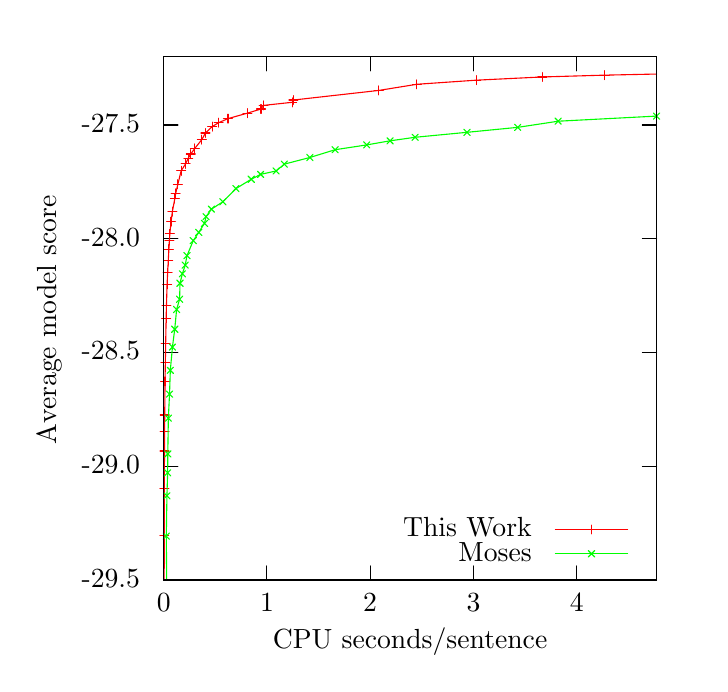
\begin{tikzpicture}[gnuplot]
%% generated with GNUPLOT 4.6p3 (Gentoo revision r0) (Lua 5.1; terminal rev. 99, script rev. 100)
%% Wed Mar 12 22:40:56 2014
\path (0.000,0.000) rectangle (8.500,8.000);
\gpcolor{color=gp lt color border}
\gpsetlinetype{gp lt border}
\gpsetlinewidth{1.00}
\draw[gp path] (1.688,0.985)--(1.868,0.985);
\draw[gp path] (7.947,0.985)--(7.767,0.985);
\node[gp node right] at (1.504,0.985) {-29.5};
\draw[gp path] (1.688,2.430)--(1.868,2.430);
\draw[gp path] (7.947,2.430)--(7.767,2.430);
\node[gp node right] at (1.504,2.430) {-29.0};
\draw[gp path] (1.688,3.875)--(1.868,3.875);
\draw[gp path] (7.947,3.875)--(7.767,3.875);
\node[gp node right] at (1.504,3.875) {-28.5};
\draw[gp path] (1.688,5.319)--(1.868,5.319);
\draw[gp path] (7.947,5.319)--(7.767,5.319);
\node[gp node right] at (1.504,5.319) {-28.0};
\draw[gp path] (1.688,6.764)--(1.868,6.764);
\draw[gp path] (7.947,6.764)--(7.767,6.764);
\node[gp node right] at (1.504,6.764) {-27.5};
\draw[gp path] (1.688,0.985)--(1.688,1.165);
\draw[gp path] (1.688,7.631)--(1.688,7.451);
\node[gp node center] at (1.688,0.677) { 0};
\draw[gp path] (2.999,0.985)--(2.999,1.165);
\draw[gp path] (2.999,7.631)--(2.999,7.451);
\node[gp node center] at (2.999,0.677) { 1};
\draw[gp path] (4.310,0.985)--(4.310,1.165);
\draw[gp path] (4.310,7.631)--(4.310,7.451);
\node[gp node center] at (4.310,0.677) { 2};
\draw[gp path] (5.622,0.985)--(5.622,1.165);
\draw[gp path] (5.622,7.631)--(5.622,7.451);
\node[gp node center] at (5.622,0.677) { 3};
\draw[gp path] (6.933,0.985)--(6.933,1.165);
\draw[gp path] (6.933,7.631)--(6.933,7.451);
\node[gp node center] at (6.933,0.677) { 4};
\draw[gp path] (1.688,7.631)--(1.688,0.985)--(7.947,0.985)--(7.947,7.631)--cycle;
\node[gp node center,rotate=-270] at (0.246,4.308) {Average model score};
\node[gp node center] at (4.817,0.215) {CPU seconds/sentence};
\node[gp node right] at (6.479,1.627) {This Work};
\gpcolor{color=gp lt color 0}
\gpsetlinetype{gp lt plot 0}
\draw[gp path] (6.663,1.627)--(7.579,1.627);
\draw[gp path] (1.694,0.985)--(1.695,1.555)--(1.696,2.142)--(1.698,2.624)--(1.700,2.874)%
  --(1.701,3.081)--(1.705,3.508)--(1.709,3.752)--(1.713,3.994)--(1.719,4.312)--(1.723,4.470)%
  --(1.731,4.742)--(1.738,4.885)--(1.746,5.040)--(1.754,5.187)--(1.760,5.296)--(1.766,5.381)%
  --(1.781,5.536)--(1.798,5.663)--(1.829,5.828)--(1.840,5.895)--(1.868,6.012)--(1.909,6.181)%
  --(1.966,6.271)--(2.000,6.343)--(2.032,6.395)--(2.084,6.468)--(2.172,6.578)--(2.218,6.662)%
  --(2.303,6.743)--(2.385,6.793)--(2.504,6.845)--(2.750,6.914)--(2.924,6.967)--(2.956,7.013)%
  --(3.320,7.052)--(3.335,7.081)--(4.420,7.203)--(4.903,7.281)--(5.656,7.333)--(6.496,7.374)%
  --(7.290,7.397)--(7.947,7.411);
\gpsetpointsize{4.00}
\gppoint{gp mark 1}{(1.695,1.555)}
\gppoint{gp mark 1}{(1.696,2.142)}
\gppoint{gp mark 1}{(1.698,2.624)}
\gppoint{gp mark 1}{(1.700,2.874)}
\gppoint{gp mark 1}{(1.701,3.081)}
\gppoint{gp mark 1}{(1.705,3.508)}
\gppoint{gp mark 1}{(1.709,3.752)}
\gppoint{gp mark 1}{(1.713,3.994)}
\gppoint{gp mark 1}{(1.719,4.312)}
\gppoint{gp mark 1}{(1.723,4.470)}
\gppoint{gp mark 1}{(1.731,4.742)}
\gppoint{gp mark 1}{(1.738,4.885)}
\gppoint{gp mark 1}{(1.746,5.040)}
\gppoint{gp mark 1}{(1.754,5.187)}
\gppoint{gp mark 1}{(1.760,5.296)}
\gppoint{gp mark 1}{(1.766,5.381)}
\gppoint{gp mark 1}{(1.781,5.536)}
\gppoint{gp mark 1}{(1.798,5.663)}
\gppoint{gp mark 1}{(1.829,5.828)}
\gppoint{gp mark 1}{(1.840,5.895)}
\gppoint{gp mark 1}{(1.868,6.012)}
\gppoint{gp mark 1}{(1.909,6.181)}
\gppoint{gp mark 1}{(1.966,6.271)}
\gppoint{gp mark 1}{(2.000,6.343)}
\gppoint{gp mark 1}{(2.032,6.395)}
\gppoint{gp mark 1}{(2.084,6.468)}
\gppoint{gp mark 1}{(2.172,6.578)}
\gppoint{gp mark 1}{(2.218,6.662)}
\gppoint{gp mark 1}{(2.303,6.743)}
\gppoint{gp mark 1}{(2.385,6.793)}
\gppoint{gp mark 1}{(2.504,6.845)}
\gppoint{gp mark 1}{(2.750,6.914)}
\gppoint{gp mark 1}{(2.924,6.967)}
\gppoint{gp mark 1}{(2.956,7.013)}
\gppoint{gp mark 1}{(3.320,7.052)}
\gppoint{gp mark 1}{(3.335,7.081)}
\gppoint{gp mark 1}{(4.420,7.203)}
\gppoint{gp mark 1}{(4.903,7.281)}
\gppoint{gp mark 1}{(5.656,7.333)}
\gppoint{gp mark 1}{(6.496,7.374)}
\gppoint{gp mark 1}{(7.290,7.397)}
\gppoint{gp mark 1}{(7.121,1.627)}
\gpcolor{color=gp lt color border}
\node[gp node right] at (6.479,1.319) {Moses};
\gpcolor{color=gp lt color 1}
\gpsetlinetype{gp lt plot 1}
\draw[gp path] (6.663,1.319)--(7.579,1.319);
\draw[gp path] (1.726,0.985)--(1.721,1.543)--(1.729,2.055)--(1.738,2.347)--(1.740,2.586)%
  --(1.747,3.040)--(1.762,3.346)--(1.772,3.648)--(1.799,3.944)--(1.828,4.170)--(1.852,4.421)%
  --(1.890,4.551)--(1.895,4.754)--(1.925,4.874)--(1.961,4.984)--(1.984,5.105)--(2.063,5.295)%
  --(2.133,5.400)--(2.206,5.515)--(2.226,5.600)--(2.294,5.695)--(2.439,5.789)--(2.605,5.956)%
  --(2.800,6.075)--(2.919,6.137)--(3.115,6.180)--(3.220,6.267)--(3.544,6.351)--(3.865,6.450)%
  --(4.266,6.511)--(4.563,6.563)--(4.881,6.608)--(5.540,6.671)--(6.184,6.734)--(6.698,6.812)%
  --(7.947,6.877);
\gppoint{gp mark 2}{(1.721,1.543)}
\gppoint{gp mark 2}{(1.729,2.055)}
\gppoint{gp mark 2}{(1.738,2.347)}
\gppoint{gp mark 2}{(1.740,2.586)}
\gppoint{gp mark 2}{(1.747,3.040)}
\gppoint{gp mark 2}{(1.762,3.346)}
\gppoint{gp mark 2}{(1.772,3.648)}
\gppoint{gp mark 2}{(1.799,3.944)}
\gppoint{gp mark 2}{(1.828,4.170)}
\gppoint{gp mark 2}{(1.852,4.421)}
\gppoint{gp mark 2}{(1.890,4.551)}
\gppoint{gp mark 2}{(1.895,4.754)}
\gppoint{gp mark 2}{(1.925,4.874)}
\gppoint{gp mark 2}{(1.961,4.984)}
\gppoint{gp mark 2}{(1.984,5.105)}
\gppoint{gp mark 2}{(2.063,5.295)}
\gppoint{gp mark 2}{(2.133,5.400)}
\gppoint{gp mark 2}{(2.206,5.515)}
\gppoint{gp mark 2}{(2.226,5.600)}
\gppoint{gp mark 2}{(2.294,5.695)}
\gppoint{gp mark 2}{(2.439,5.789)}
\gppoint{gp mark 2}{(2.605,5.956)}
\gppoint{gp mark 2}{(2.800,6.075)}
\gppoint{gp mark 2}{(2.919,6.137)}
\gppoint{gp mark 2}{(3.115,6.180)}
\gppoint{gp mark 2}{(3.220,6.267)}
\gppoint{gp mark 2}{(3.544,6.351)}
\gppoint{gp mark 2}{(3.865,6.450)}
\gppoint{gp mark 2}{(4.266,6.511)}
\gppoint{gp mark 2}{(4.563,6.563)}
\gppoint{gp mark 2}{(4.881,6.608)}
\gppoint{gp mark 2}{(5.540,6.671)}
\gppoint{gp mark 2}{(6.184,6.734)}
\gppoint{gp mark 2}{(6.698,6.812)}
\gppoint{gp mark 2}{(7.947,6.877)}
\gppoint{gp mark 2}{(7.121,1.319)}
\gpcolor{color=gp lt color border}
\gpsetlinetype{gp lt border}
\draw[gp path] (1.688,7.631)--(1.688,0.985)--(7.947,0.985)--(7.947,7.631)--cycle;
%% coordinates of the plot area
\gpdefrectangularnode{gp plot 1}{\pgfpoint{1.688cm}{0.985cm}}{\pgfpoint{7.947cm}{7.631cm}}
\end{tikzpicture}
%% gnuplot variables
\\%
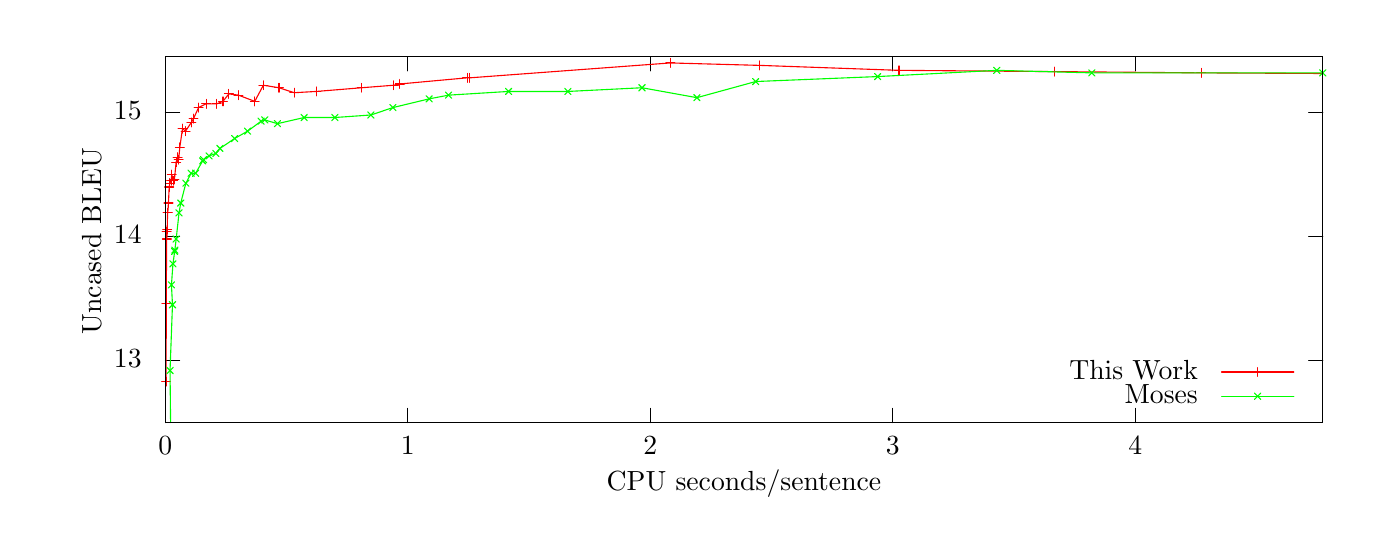
\begin{tikzpicture}[gnuplot]
%% generated with GNUPLOT 4.6p3 (Gentoo revision r0) (Lua 5.1; terminal rev. 99, script rev. 100)
%% Wed Mar 12 22:06:18 2014
\path (0.000,0.000) rectangle (17.000,6.000);
\gpcolor{color=gp lt color border}
\gpsetlinetype{gp lt border}
\gpsetlinewidth{1.00}
\draw[gp path] (1.748,1.772)--(1.928,1.772);
\draw[gp path] (16.447,1.772)--(16.267,1.772);
\node[gp node right] at (1.564,1.772) {13};
\draw[gp path] (1.748,3.347)--(1.928,3.347);
\draw[gp path] (16.447,3.347)--(16.267,3.347);
\node[gp node right] at (1.564,3.347) {14};
\draw[gp path] (1.748,4.922)--(1.928,4.922);
\draw[gp path] (16.447,4.922)--(16.267,4.922);
\node[gp node right] at (1.564,4.922) {15};
\draw[gp path] (1.748,0.985)--(1.748,1.165);
\draw[gp path] (1.748,5.631)--(1.748,5.451);
\node[gp node center] at (1.748,0.677) { 0};
\draw[gp path] (4.827,0.985)--(4.827,1.165);
\draw[gp path] (4.827,5.631)--(4.827,5.451);
\node[gp node center] at (4.827,0.677) { 1};
\draw[gp path] (7.907,0.985)--(7.907,1.165);
\draw[gp path] (7.907,5.631)--(7.907,5.451);
\node[gp node center] at (7.907,0.677) { 2};
\draw[gp path] (10.986,0.985)--(10.986,1.165);
\draw[gp path] (10.986,5.631)--(10.986,5.451);
\node[gp node center] at (10.986,0.677) { 3};
\draw[gp path] (14.066,0.985)--(14.066,1.165);
\draw[gp path] (14.066,5.631)--(14.066,5.451);
\node[gp node center] at (14.066,0.677) { 4};
\draw[gp path] (1.748,5.631)--(1.748,0.985)--(16.447,0.985)--(16.447,5.631)--cycle;
\node[gp node center,rotate=-270] at (0.858,3.308) {Uncased BLEU};
\node[gp node center] at (9.097,0.215) {CPU seconds/sentence};
\node[gp node right] at (14.979,1.627) {This Work};
\gpcolor{color=gp lt color 0}
\gpsetlinetype{gp lt plot 0}
\draw[gp path] (15.163,1.627)--(16.079,1.627);
\draw[gp path] (1.757,1.505)--(1.761,2.497)--(1.764,3.410)--(1.768,3.316)--(1.772,3.442)%
  --(1.777,3.647)--(1.779,3.647)--(1.788,3.773)--(1.797,3.977)--(1.806,4.025)--(1.821,4.056)%
  --(1.830,4.135)--(1.849,4.056)--(1.864,4.072)--(1.885,4.292)--(1.904,4.355)--(1.918,4.324)%
  --(1.932,4.481)--(1.966,4.718)--(2.005,4.686)--(2.078,4.796)--(2.106,4.844)--(2.170,4.985)%
  --(2.266,5.033)--(2.401,5.033)--(2.480,5.064)--(2.555,5.159)--(2.677,5.143)--(2.884,5.064)%
  --(2.993,5.269)--(3.192,5.237)--(3.385,5.174)--(3.665,5.190)--(4.242,5.237)--(4.650,5.269)%
  --(4.726,5.285)--(5.581,5.363)--(5.616,5.363)--(8.163,5.552)--(9.299,5.521)--(11.066,5.458)%
  --(13.039,5.442)--(14.903,5.426)--(16.447,5.418);
\gpsetpointsize{4.00}
\gppoint{gp mark 1}{(1.757,1.505)}
\gppoint{gp mark 1}{(1.761,2.497)}
\gppoint{gp mark 1}{(1.764,3.410)}
\gppoint{gp mark 1}{(1.768,3.316)}
\gppoint{gp mark 1}{(1.772,3.442)}
\gppoint{gp mark 1}{(1.777,3.647)}
\gppoint{gp mark 1}{(1.779,3.647)}
\gppoint{gp mark 1}{(1.788,3.773)}
\gppoint{gp mark 1}{(1.797,3.977)}
\gppoint{gp mark 1}{(1.806,4.025)}
\gppoint{gp mark 1}{(1.821,4.056)}
\gppoint{gp mark 1}{(1.830,4.135)}
\gppoint{gp mark 1}{(1.849,4.056)}
\gppoint{gp mark 1}{(1.864,4.072)}
\gppoint{gp mark 1}{(1.885,4.292)}
\gppoint{gp mark 1}{(1.904,4.355)}
\gppoint{gp mark 1}{(1.918,4.324)}
\gppoint{gp mark 1}{(1.932,4.481)}
\gppoint{gp mark 1}{(1.966,4.718)}
\gppoint{gp mark 1}{(2.005,4.686)}
\gppoint{gp mark 1}{(2.078,4.796)}
\gppoint{gp mark 1}{(2.106,4.844)}
\gppoint{gp mark 1}{(2.170,4.985)}
\gppoint{gp mark 1}{(2.266,5.033)}
\gppoint{gp mark 1}{(2.401,5.033)}
\gppoint{gp mark 1}{(2.480,5.064)}
\gppoint{gp mark 1}{(2.555,5.159)}
\gppoint{gp mark 1}{(2.677,5.143)}
\gppoint{gp mark 1}{(2.884,5.064)}
\gppoint{gp mark 1}{(2.993,5.269)}
\gppoint{gp mark 1}{(3.192,5.237)}
\gppoint{gp mark 1}{(3.385,5.174)}
\gppoint{gp mark 1}{(3.665,5.190)}
\gppoint{gp mark 1}{(4.242,5.237)}
\gppoint{gp mark 1}{(4.650,5.269)}
\gppoint{gp mark 1}{(4.726,5.285)}
\gppoint{gp mark 1}{(5.581,5.363)}
\gppoint{gp mark 1}{(5.616,5.363)}
\gppoint{gp mark 1}{(8.163,5.552)}
\gppoint{gp mark 1}{(9.299,5.521)}
\gppoint{gp mark 1}{(11.066,5.458)}
\gppoint{gp mark 1}{(13.039,5.442)}
\gppoint{gp mark 1}{(14.903,5.426)}
\gppoint{gp mark 1}{(15.621,1.627)}
\gpcolor{color=gp lt color border}
\node[gp node right] at (14.979,1.319) {Moses};
\gpcolor{color=gp lt color 1}
\gpsetlinetype{gp lt plot 1}
\draw[gp path] (15.163,1.319)--(16.079,1.319);
\draw[gp path] (1.815,0.985)--(1.808,1.646)--(1.839,2.481)--(1.826,2.733)--(1.845,3.001)%
  --(1.867,3.158)--(1.869,3.174)--(1.886,3.316)--(1.922,3.647)--(1.944,3.773)--(2.009,4.025)%
  --(2.076,4.151)--(2.133,4.151)--(2.222,4.308)--(2.234,4.324)--(2.304,4.371)--(2.390,4.403)%
  --(2.442,4.466)--(2.628,4.592)--(2.793,4.686)--(2.965,4.812)--(3.011,4.828)--(3.172,4.781)%
  --(3.512,4.859)--(3.902,4.859)--(4.359,4.891)--(4.638,4.985)--(5.099,5.096)--(5.345,5.143)%
  --(6.107,5.190)--(6.860,5.190)--(7.802,5.237)--(8.499,5.111)--(9.246,5.316)--(10.795,5.379)%
  --(12.307,5.458)--(13.514,5.426)--(16.447,5.426);
\gppoint{gp mark 2}{(1.808,1.646)}
\gppoint{gp mark 2}{(1.839,2.481)}
\gppoint{gp mark 2}{(1.826,2.733)}
\gppoint{gp mark 2}{(1.845,3.001)}
\gppoint{gp mark 2}{(1.867,3.158)}
\gppoint{gp mark 2}{(1.869,3.174)}
\gppoint{gp mark 2}{(1.886,3.316)}
\gppoint{gp mark 2}{(1.922,3.647)}
\gppoint{gp mark 2}{(1.944,3.773)}
\gppoint{gp mark 2}{(2.009,4.025)}
\gppoint{gp mark 2}{(2.076,4.151)}
\gppoint{gp mark 2}{(2.133,4.151)}
\gppoint{gp mark 2}{(2.222,4.308)}
\gppoint{gp mark 2}{(2.234,4.324)}
\gppoint{gp mark 2}{(2.304,4.371)}
\gppoint{gp mark 2}{(2.390,4.403)}
\gppoint{gp mark 2}{(2.442,4.466)}
\gppoint{gp mark 2}{(2.628,4.592)}
\gppoint{gp mark 2}{(2.793,4.686)}
\gppoint{gp mark 2}{(2.965,4.812)}
\gppoint{gp mark 2}{(3.011,4.828)}
\gppoint{gp mark 2}{(3.172,4.781)}
\gppoint{gp mark 2}{(3.512,4.859)}
\gppoint{gp mark 2}{(3.902,4.859)}
\gppoint{gp mark 2}{(4.359,4.891)}
\gppoint{gp mark 2}{(4.638,4.985)}
\gppoint{gp mark 2}{(5.099,5.096)}
\gppoint{gp mark 2}{(5.345,5.143)}
\gppoint{gp mark 2}{(6.107,5.190)}
\gppoint{gp mark 2}{(6.860,5.190)}
\gppoint{gp mark 2}{(7.802,5.237)}
\gppoint{gp mark 2}{(8.499,5.111)}
\gppoint{gp mark 2}{(9.246,5.316)}
\gppoint{gp mark 2}{(10.795,5.379)}
\gppoint{gp mark 2}{(12.307,5.458)}
\gppoint{gp mark 2}{(13.514,5.426)}
\gppoint{gp mark 2}{(16.447,5.426)}
\gppoint{gp mark 2}{(15.621,1.319)}
\gpcolor{color=gp lt color border}
\gpsetlinetype{gp lt border}
\draw[gp path] (1.748,5.631)--(1.748,0.985)--(16.447,0.985)--(16.447,5.631)--cycle;
%% coordinates of the plot area
\gpdefrectangularnode{gp plot 1}{\pgfpoint{1.748cm}{0.985cm}}{\pgfpoint{16.447cm}{5.631cm}}
\end{tikzpicture}
%% gnuplot variables

\end{tabular}
\end{figure*}

\subsection{Priority Queue}
Search proceeds in a best-first fashion controlled by a priority queue.  For each source phrase, we convert the compatible hypotheses into a trie.  The target phrases were already converted into a trie when the phrase table was loaded.  We then push the root $(\epsilon, \epsilon)$ boundary pair into the priority queue.  We do this for all source phrases under consideration, putting their root boundary pairs into the same priority queue.  The algorithm then loops by popping the top boundary pair.  It the top boundary pair uniquely describes a hypothesis and target phrase then remaining features are evaluated and the new hypothesis is output to the decoder's stack.  Otherwise, the algorithm splits the boundary pair and pushes both split versions.  Iteration continues until $k$ new hypotheses have been found.  

\subsection{Overall Algorithm}
We build hypotheses from left-to-right and manage stacks just like cube pruning. The only difference is how the $k$ elements of these stacks are selected.  

When the decoder matches a hypothesis with a compatible source phrase, we immediately evaluate the distortion feature and update future costs.  Our future costs are exactly the same as those used in Moses \cite{moses}: the highest-scoring way to cover the rest of the source sentence.  This includes the language model score within target phrases but ignores the change in language model score that would occur were these phrases to be appended together.  The hypotheses compatible with each source phrase are arranged into a trie.  Finally, the priority queue algorithm from the preceding section searches for options that the language model likes.    

\section{Experiments}
The primary claim is that our algorithm performs better than cube pruning in terms of the trade-off between time and accuracy.  To test this claim, we compare our new decoder implementation with Moses \cite{moses}.  


%We measure performance by translating a Chinese-English test set of 1677 sentences. This data is a subset of development data prepared for the BOLT Chinese-English translation task, and consists of translated Chinese online text sources, such as discussion forums. We trained our phrase table using a bitext of 10.8 million sentence pairs, which after tokenization amounts to approximately 290 million words on the English side. The bitext contains data from several sources, including news articles, UN proceedings, Hong Kong government documents, online forum data, and specialized sources such as an idiom translation table. Our language model was also trained using the English half of this bitext, using modified Kneser-Ney smoothing \cite{}. 

%We trained weights for our translation system using the Phrasal toolkit, using the online Adagrad technique to minimize a smoothed version of BLEU\cite{}. All our translation models used a simple feature set consisting of forward and backward translation models, a language model, a target word generation penalty and a linear distortion feature.  

We used a basic phrase-based Chinese--English system for the NIST Open MT 2012 evaluation with standard phrase table features, the distortion feature, and a single language model.  The reordering limit was set to 15.   The phrase table was pre-filtered to at most 20 target-side phrases per source phrase using the same method as Moses uses internally; we then disabled these limits in the individual decoders to ensure a consistent set of target phrases.  We vary the pop limit $k$ and also set the Moses stack size to $k$ to disable this second form of pruning.  This system is not designed to be competitive, but rather a benchmark that removes as many confounds as possible.

Moses \cite{moses} revision d6df825 was compiled with all optimizations recommended in the documentation.  We use the in-memory phrase table for speed.  Tests were run on otherwise-idle identical machines with 32 GB RAM; the processes did not come close to running out of memory.  Binarized KenLM language models in probing format were placed in a RAM disk and text phrase tables were forced into the disk cache before each run.  Timing is based on CPU usage reported by the kernel (user plus system) minus loading time, as measured by running on empty input; our decoder is also faster at loading.  All results are single-threaded.  Model score is averaged over all 1677 sentences; higher is better.  We have verified that the model scores are comparable across decoders through short sentences and $K$-best list agreement.

\section{Conclusion}
%TODO
When the decoder matches a hypothesis with a compatible source phrase, we immediately evaluate the distortion feature and update future costs.  Our future costs are exactly the same as those used in Moses \cite{moses}: the highest-scoring way to cover the rest of the source sentence.  This includes the language model score within target phrases but ignores the change in language model score that would occur were these phrases to be appended together.  The hypotheses compatible with each source phrase are arranged into a trie and the language model algorithm searches for good combinations of hypotheses and target phrases.


\bibliographystyle{acl}
\bibliography{paper}
\end{document}
